\whiteBGstarBegin
\setcounter{section}{0}
\begin{enumerate}[label=\bfseries Câu \arabic*:]
	
	\item \mkstar{1} [4]
	
	\cauhoi{
		Quá trình biến đổi trạng thái trong đó nhiệt độ được giữ không đổi là quá trình
		\begin{mcq}(4)
			\item đẳng nhiệt.
			\item đẳng tích.
			\item đẳng áp.
			\item đoạn nhiệt.
		\end{mcq}
	}
	
	\loigiai{
		\textbf{Đáp án: A.}
		
		Quá trình biến đổi trạng thái trong đó nhiệt độ được giữ không đổi là quá trình đẳng nhiệt.
	}
	
	\item \mkstar{1} [5]
	
	\cauhoi{
		Biểu thức $p_1V_1=p_2V_2$ biểu diễn quá trình
		\begin{mcq}(2)
			\item đẳng áp và đẳng nhiệt. 
			\item đẳng áp.
			\item đẳng tích.
			\item đẳng nhiệt.
		\end{mcq}
		
	}
	
	\loigiai{
		\textbf{Đáp án: D.}
		
		Biểu thức $p_1V_1=p_2V_2$ biểu diễn quá trình đẳng nhiệt.
	}
	
	\item \mkstar{1} [5]
	
	\cauhoi{
		Công thức nào sau đây liên quan đến quá trình đẳng nhiệt?
		\begin{mcq}(4)
			\item $\dfrac{V}{T} = \text{hằng số}$. 
			\item $pV=\text{hằng số}$.
			\item $\dfrac{p}{T} = \text{hằng số}$.
			\item $\dfrac{p}{V} = \text{hằng số}$.
		\end{mcq}
	}
	
	\loigiai{\textbf{Đáp án: B.}		
		
		Công thức liên quan đến quá trình đẳng nhiệt là $pV=\text{hằng số}$.
		
	}

	\item \mkstar{1} [24]
	
	\cauhoi{
		Hệ thức nào sau đây là của định luật Boyle - Mariotte?
		\begin{mcq}(4)
			\item $p_1V_2=p_2V_1$. 
			\item $\dfrac{p}{V} = \text{hằng số}$.
			\item $pV=\text{hằng số}$.
			\item $\dfrac{V}{p}=\text{hằng số}$.
		\end{mcq}
	}
	
	\loigiai{\textbf{Đáp án: C.}		
		
		Hệ thức của định luật Boyle - Mariotte là $pV=\text{hằng số}$, khi áp dụng cho quá trình biến đổi từ (1) sang (2) là $p_1V_1=p_2V_2$. 
		
	}

	\item \mkstar{1} [5]
	
	\cauhoi{
		\begin{minipage}[l]{0.7\textwidth}
			Đồ thị bên biểu diễn hai đường đẳng nhiệt của cùng một lượng khí lí tưởng. Mối quan hệ về nhiệt độ của hai đường đẳng nhiệt này là
			\begin{mcq}(2)
				\item $T_2 > T_1$. 
				\item $T_2 = T_1$.
				\item $T_2 < T_1$.
				\item $T_2 \leq T_1$.
			\end{mcq}
		\end{minipage}
		\begin{minipage}[r]{0.3\textwidth}
			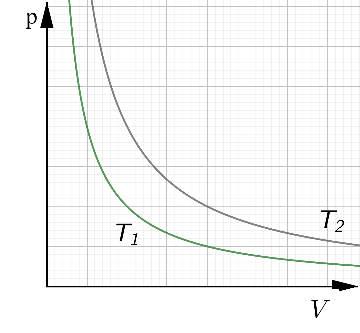
\includegraphics[scale=1.2]{../figs/VN10-2021-PH-TP030-1}
		\end{minipage}
		
	}
	
	\loigiai{\textbf{Đáp án: A.}		
		
		Trong hệ tọa độ (O$pV$), đường đẳng nhiệt ở trên ứng với nhiệt độ cao hơn.
		
	}

		\item \mkstar{1} [29]
	
	\cauhoi{
		Đường biểu diễn sự biến thiên của áp suất theo thể tích khi nhiệt độ không thay đổi gọi là đường đẳng nhiệt. Trong hệ tọa độ (O$pV$) đường đẳng nhiệt có dạng là
		\begin{mcq}
			\item đường thẳng kéo dài đi qua gốc tọa độ O. 
			\item parabol.
			\item hyperbol.
			\item đường thẳng kéo dài song song với trục hoành $\text{O}V$.
		\end{mcq}
	}
	
	\loigiai{\textbf{Đáp án: C.}		
		
		Trong hệ tọa độ (O$pV$) đường đẳng nhiệt có dạng hyperbol.
		
	}

	\item \mkstar{2} [5]
	
	\cauhoi{
		Một lượng khí ở nhiệt độ không đổi $\SI{20}{\celsius}$, thể tích $\SI{2}{m^3}$, áp suất $\SI{2}{atm}$. Nếu áp suất giảm còn $\SI{1}{atm}$ thì thể tích khối khí là bao nhiêu?
		\begin{mcq}(4)
			\item $\SI{4}{m^3}$. 
			\item $\SI{1}{m^3}$.
			\item $\SI{2}{m^3}$.
			\item $\SI{0.5}{m^3}$.
		\end{mcq}
	}
	
	\loigiai{\textbf{Đáp án: A.}		

		Vì nhiệt độ là không đổi nên quá trình là đẳng nhiệt. Áp dụng phương trình:
		$$p_1V_1=p_2V_2 \Rightarrow V_2 = \SI{4}{m^3}.$$
	}
	
	

	\item \mkstar{2} [5]
	
	\cauhoi{
		Một khối khí lí tưởng có thể tích 5 lít, đang ở áp suất $\SI{6}{atm}$ thì dãn nở đẳng nhiệt, áp suất giảm còn $\SI{1.5}{atm}$. Thể tích của khối khí sau khi dãn bằng
		\begin{mcq}(4)
			\item $\SI{20}{l}$.
			\item $\SI{10}{l}$.
			\item $\SI{15}{l}$.
			\item $\SI{1.25}{l}$.
		\end{mcq}
	}
	
	\loigiai{\textbf{Đáp án: A.}		
		
		Vì quá trình là đẳng nhiệt nên ta có phương trình:
		
				$$p_1V_1=v_2V_2 \Rightarrow V_2 = \SI{20}{l}.$$
	}

	

	

	\item \mkstar{2} [29]
	
	\cauhoi{
		Dưới áp suất $p$ một lượng khí có thể tích là 5 lít. Tính thể tích của lượng khí này khi áp suất giảm đi 3 lần so với ban đầu. Biết nhiệt độ được giữ không đổi.
		\begin{mcq}(4)
			\item 15 lít.
			\item 20 lít.
			\item 2,5 lít.
			\item 7,5 lít.
		\end{mcq}
	}
	
	\loigiai{\textbf{Đáp án: A.}		
		
		
		Vì quá trình là đẳng nhiệt nên ta có phương trình:
		
		$$p_1V_1=p_2V_2 \Rightarrow V_2 =\dfrac{p_1}{p_2}V_1 = \dfrac{1}{\dfrac{1}{3}}V_1 = 3V_1= \SI{15}{l}.$$
	}

		\item \mkstar{1} [7]
	
	\cauhoi{
		Phát biểu và viết biểu thức của định luật Bôi-lơ - Ma-ri-ốt (không cần chú thích các đại lượng). Vẽ đường đẳng nhiệt trong hệ tọa độ $\text{O}pV$.
	}
	
	\loigiai{
		Phát biểu:
		\begin{itemize}
			\item Cách 1: Ở nhiệt độ không đổi, tích áp suất và thể tích của một lượng khí lí tưởng xác định là một hằng số;
			\item Cách 2: Trong quá trình đẳng nhiệt của một lượng khí lí tưởng xác định, áp suất tỉ lệ nghịch với thể tích.
		\end{itemize}
		Biểu thức:
		\begin{itemize}
			\item Cách 1: $pV = \text{hằng số}$;
			\item Cách 2: $p_1V_1 = p_2V_2$;
			\item Cách 3: $p\sim \dfrac{1}{V}$.
		\end{itemize}
		Đồ thị:
		
		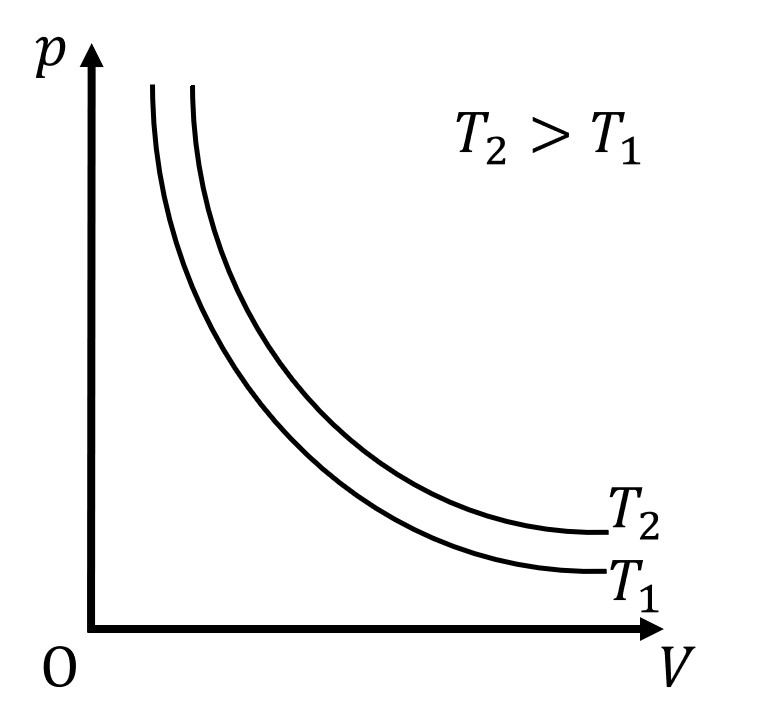
\includegraphics[scale=0.4]{../figs/VN10-PH-37-L-027-1-1-1.jpg}
	}
	
	\item \mkstar{1} [9]
	
	\cauhoi{
		Quá trình đẳng nhiệt là gì?
	}
	
	\loigiai{
		Quá trình đẳng nhiệt là quá trình biến đổi trạng thái mà trong đó nhiệt độ không thay đổi.
	}

	
	\item \mkstar{2} [4]
	
	\cauhoi{
		\begin{enumerate}[label=\alph*)]
			\item Một lượng khí lí tưởng ở trạng thái (1): $p_1=\SI{e5}{Pa}$, $V_1=\SI{30}{l}$. Người ta nén đẳng nhiệt thể tích giảm xuống còn $\SI{20}{l}$. Tính áp suất của chất khí sau khi nén.
			\item Một chất khí lí tưởng ở trạng thái có áp suất $\SI{4e5}{Pa}$, thể tích là $\SI{25}{cm^3}$. Nếu áp suất của chất khí giảm xuống còn $\SI{0.5e5}{Pa}$ thì thể tích khí là bao nhiêu?
		\end{enumerate}
	}
	
	\loigiai{
		\begin{enumerate}[label=\alph*)]
			\item Đẳng nhiệt (1): $p_1=\SI{e5}{Pa}$, $V_1=\SI{30}{l}$ sang (2): $V_2=\SI{20}{l}$, $p_2=?$
			
			Vì quá trình là đẳng nhiệt nên ta có phương trình:
			
			$$p_1V_1=p_2V_2 \Rightarrow p_2 =\dfrac{V_1}{V_2}p_1 = \SI{1.5e5}{Pa}.$$
			
			\item Đẳng nhiệt $p_1=\SI{4e5}{Pa}$, $V_1=\SI{25}{cm^3}$ sang (2): $p_2=\SI{0.5e5}{Pa}$, $V_2=?$
			
			Vì quá trình là đẳng nhiệt nên ta có phương trình:
			
			$$p_1V_1=p_2V_2 \Rightarrow V_2 =\dfrac{p_1}{p_2}V_1 = \SI{200}{cm^3}.$$
			
		\end{enumerate}
	}
	
	
	\item \mkstar{2} [6]
	
	\cauhoi{
		Nghề thợ lặn là một nghề nguy hiểm và yêu cầu phải có sức khỏe cực tốt đặc biệt là khi lặn sâu xuông nước. Cho rằng khi lặn nhiệt độ của nước là không đổi. Bằng kiến thức Vật lý Nhiệt học đã học, em hãy giải thích nguyên nhân dẫn đến nguy hiểm mà người thợ lặn gặp phải.
	}
	
	\loigiai{
		Khi người thợ lặn lặn sâu xuống nước thì áp suất nước tăng ($p$ tăng), mà nhiệt độ của quá trình coi như không đổi, theo định luật Boyle - Mariotte thì $p$ tăng $V$ giảm, khiến phổi người thợ lặn bị co bóp mạnh và gây ra nguy hiểm.
	}

	\item \mkstar{2} [6]
	
	\cauhoi{
		Dưới áp suất $\SI{2e4}{N/m^2}$, một lượng khí có thể tích $\SI{20}{l}$. Tính thể tích của lượng khí đó dưới áp suất $\SI{4e4}{N/m^2}$, coi nhiệt độ không đổi.
	}
	
	\loigiai{
		
		Vì quá trình là đẳng nhiệt nên ta có phương trình:
		
		$$p_1V_1=p_2V_2 \Rightarrow V_2 =\dfrac{p_1}{p_2}V_1 = \SI{10}{l}.$$
	}



	\item \mkstar{2} [11]
	
	\cauhoi{
		Một lượng khí có thể tích $\SI{20}{l}$ và áp suất $\SI{1}{atm}$. Nén đẳng nhiệt khí tới áp suất $\SI{4}{atm}$. Tính thể tích của khí sau khi nén.
	}
	
	\loigiai{
		Đẳng nhiệt (1): $p_1=\SI{1}{atm}$, $V_1=\SI{20}{l}$ sang (2): $V_2=?$, $p_2=\SI{4}{atm}$
		
		Vì quá trình là đẳng nhiệt nên ta có phương trình:
		
		$$p_1V_1=p_2V_2 \Rightarrow V_2 =\dfrac{p_1}{p_2}V_1 = \SI{5}{l}.$$
	}

	\item \mkstar{2} [13]
	
	\cauhoi{
		Một lượng khí trong xi lanh ban đầu có thể tích $V_1=\SI{10}{l}$, nhiệt độ $\SI{227}{\celsius}$, áp suất $p_1=\SI{4}{atm}$ được dãn nở đẳng nhiệt để áp suất giảm 2 lần. Xác định thể tích của lượng khí sau khi nén.
	}
	
	\loigiai{
		
		Đẳng nhiệt (1): $p_1=\SI{4}{atm}$, $V_1=\SI{10}{l}$ sang (2): $V_2=?$, $p_2=\SI{2}{atm}$
		
		Vì quá trình là đẳng nhiệt nên ta có phương trình:
		
		$$p_1V_1=p_2V_2 \Rightarrow V_2 =\dfrac{p_1}{p_2}V_1 = \SI{20}{l}.$$
	}



	\item \mkstar{2} [17]
	
	\cauhoi{
		Một xi-lanh chứa $\SI{150}{cm^3}$ khí ở áp suất $\SI{2e5}{Pa}$. Pit-tông nén khí trong xi-lanh xuống còn $\SI{100}{cm^3}$. Tính áp suất của khí trong xi-lanh lúc này, coi nhiệt độ không đổi.
	}
	
	\loigiai{
		
		Đẳng nhiệt (1): $p_1=\SI{2e5}{Pa}$, $V_1=\SI{150}{cm^3}$ sang (2): $V_2=\SI{100}{cm^3}$, $p_2=?$
		
		Vì quá trình là đẳng nhiệt nên ta có phương trình:
		
		$$p_1V_1=p_2V_2 \Rightarrow p_2 =\dfrac{V_1}{V_2}p_1 = \SI{3e5}{Pa}.$$
	}

	\item \mkstar{2} [18]
	
	\cauhoi{
		Nén khí đẳng nhiệt từ thể tích 18 lít đến thể tích 6 lít thì áp suất tăng thêm một lượng $\Delta p = \SI{60}{kPa}$. Áp suất ban đầu của khí đó là bao nhiêu?
	}
	
	\loigiai{
		
		Đẳng nhiệt (1): $p_1$, $V_1=\SI{18}{l}$ sang (2): $V_2=\SI{6}{l}$, $p_2=p_1+\SI{60}{kPa}$
		
		Vì quá trình là đẳng nhiệt nên ta có phương trình:
		
		$$p_1V_1=p_2V_2 \Rightarrow p_1 = \SI{30}{kPa}.$$
	}

	\item \mkstar{2} [19]
	
	\cauhoi{
		Một khối khí lí tưởng có thể tích $\SI{4}{cm^3}$, áp suất $\SI{8}{atm}$ và nhiệt độ $\SI{27}{\celsius}$. Sau quá trình biến đổi trạng thái người ta thấy nhiệt độ của khối khí không đổi nhưng thể tích của khối khí là $\SI{5}{cm^3}$. Tính áp suất của khối khí sau quá trình biến đổi.
	}
	
	\loigiai{
		
		Đẳng nhiệt (1): $p_1=\SI{8}{atm}$, $V_1=\SI{4}{cm^3}$ sang (2): $V_2=\SI{5}{cm^3}$, $p_2=?$
		
		Vì quá trình là đẳng nhiệt nên ta có phương trình:
		
		$$p_1V_1=p_2V_2 \Rightarrow p_2 =\dfrac{V_1}{V_2}p_1 = \SI{6.4}{atm}.$$
	}

	\item \mkstar{2} [19]
	
	\cauhoi{
		Một khối khí được nén từ thể tích 16 lít xuống còn 8 lít, khi đó áp suất của khí tăng thêm $\SI{0.5}{atm}$. Tìm áp suất ban đầu của khí biết trong quá trình nén, nhiệt độ được giữ không đổi.
	}
	
	\loigiai{
		Đẳng nhiệt (1): $p_1$, $V_1=\SI{16}{l}$ sang (2): $V_2=\SI{8}{l}$, $p_2=p_1+\SI{0.5}{atm}$
		
		Vì quá trình là đẳng nhiệt nên ta có phương trình:
		
		$$p_1V_1=p_2V_2 \Rightarrow p_1 = \SI{0.5}{atm}.$$
	}

	\item \mkstar{2} [28]
	
	\cauhoi{
		Một lượng khí được nén đẳng nhiệt từ thể tích 10 lít còn 4 lít, khi đó áp suất tăng thêm $\SI{1.5}{atm}$. Áp suất khí ban đầu là bao nhiêu?
	}
	
	\loigiai{
		Đẳng nhiệt (1): $p_1$, $V_1=\SI{10}{l}$ sang (2): $V_2=\SI{4}{l}$, $p_2=p_1+\SI{1.5}{atm}$
		
		Vì quá trình là đẳng nhiệt nên ta có phương trình:
		
		$$p_1V_1=p_2V_2 \Rightarrow p_1 = \SI{1}{atm}.$$
	}


	\item \mkstar{2} [31]
	
	\cauhoi{
		Khi có thể tích 5 lít, áp suất $\SI{2}{atm}$. Giữ nhiệt độ khí không đổi và giảm thể tích xuống còn 2 lít. Tính áp suất khí lúc này.
	}
	
	\loigiai{
		Đẳng nhiệt (1): $p_1=\SI{2}{atm}$, $V_1=\SI{5}{l}$ sang (2): $V_2=\SI{2}{l}$, $p_2=?$
		
		Vì quá trình là đẳng nhiệt nên ta có phương trình:
		
		$$p_1V_1=p_2V_2 \Rightarrow p_2 =\dfrac{V_1}{V_2}p_1 = \SI{5}{atm}.$$
		
	}

	\item \mkstar{2} [32]
	
	\cauhoi{
		Quan sát người thợ lặn dưới một hồ nước người ta nhận thấy các bọt khí tạo ra càng lúc càng to lên khi tiến gần đến mặt nước. Em hãy dùng định luật Boyle Mariotte để giải thích hiện tượng trên. Xem nhiệt độ của nước là như nhau tại mọi nơi trong hồ nước.
	}
	
	\loigiai{
		Do quá trình là đẳng nhiệt, áp suất tỉ lệ nghịch với thể tích khí. Càng gần mặt nước thì áp suất càng giảm, do đó thể tích càng tăng, nên bong bóng càng to ra.
		
	}
	\item \mkstar{3} [15]

\cauhoi{
	Người ta bơm khí vào một quả bóng có dung tích $\SI{3}{l}$. Mỗi lần bơm được $\SI{300}{cm^3}$ khí ở áp suất $\SI{1}{atm}$ vào bên trong quả bóng. Vỏ bóng chịu được áp suất tối đa là $\SI{2.5}{atm}$. Sau 20 lần bơm, quả bóng có bị nổ không? Tại sao? Cho rằng nhiệt độ không thay đổi trong suốt quá trình bơm và trước khi bơm trong quả bóng không có không khí.
}

\loigiai{
	Đổi $\Delta V = \SI{300}{cm^3} = \SI{0.3}{l}$.
	
	Sau 20 lần bơm thì $\Delta V_{20} = 20\Delta V = \SI{6}{l}$.
	
	Xem quá trình như là đẳng nhiệt nén lượng không khí từ bên ngoài (20 lần bơm) nén vào trong 1 quả bóng có thể tích 3 lít: (1): $p_1=\SI{1}{atm}$, $V_1=\SI{6}{l}$ sang (2): $V_2=\SI{3}{l}$, $p_2=?$
	
	Vì quá trình là đẳng nhiệt nên ta có phương trình:
	
	$$p_1V_1=p_2V_2 \Rightarrow p_2 =\dfrac{V_1}{V_2}p_1 = \SI{2}{atm}.$$
	
	Quả bóng chịu được áp suất tối đa là $\SI{2.5}{atm}$ nên không phát nổ.
}

\item \mkstar{3} [29]

\cauhoi{
	Nén khí đẳng nhiệt từ thể tích 6 lít đến thể tích 9 lít thì áp suất thay đổi một lượng bằng $\SI{2.5}{atm}$. Tính áp suất ban đầu của khối khí này.
}

\loigiai{
	Vì áp suất tỉ lệ nghịch với thể tích nên thể tích tăng thì áp suất giảm, dẫn đến $p_2=p_1-\Delta p$.
	
	Quá trình đẳng nhiệt (1): $p_1$, $V_1=\SI{6}{l}$ sang (2): $V_2=\SI{9}{l}$, $p_2=p_1-\SI{2.5}{atm}$
	
	Vì quá trình là đẳng nhiệt nên ta có phương trình:
	
	$$p_1V_1=p_2V_2 \Rightarrow p_1 = \SI{7.5}{atm}.$$
}
\end{enumerate}
\whiteBGstarEnd